%-------------------------------------------------------------------------------
% seq66 setmaster
%-------------------------------------------------------------------------------
%
% \file        seq66 setmaster.tex
% \library     Documents
% \author      Chris Ahlstrom
% \date        2020-01-13
% \update      2020-01-18
% \version     $Revision$
% \license     $XPC_GPL_LICENSE$
%
%     Provides a discussion of the MIDI GUI setmaster that Seq66
%     supports.
%
%-------------------------------------------------------------------------------

\section{Seq66 Set Master}
\label{sec:setmaster}

   The \textbf{Set Master} is a way to get a global view of all the screensets in
   a \textsl{Seq66} MIDI file, and to be able to do some simple operations
   (movement, naming, etc.) with the sets.  It is still a work in progress.

\begin{figure}[H]
   \centering 
   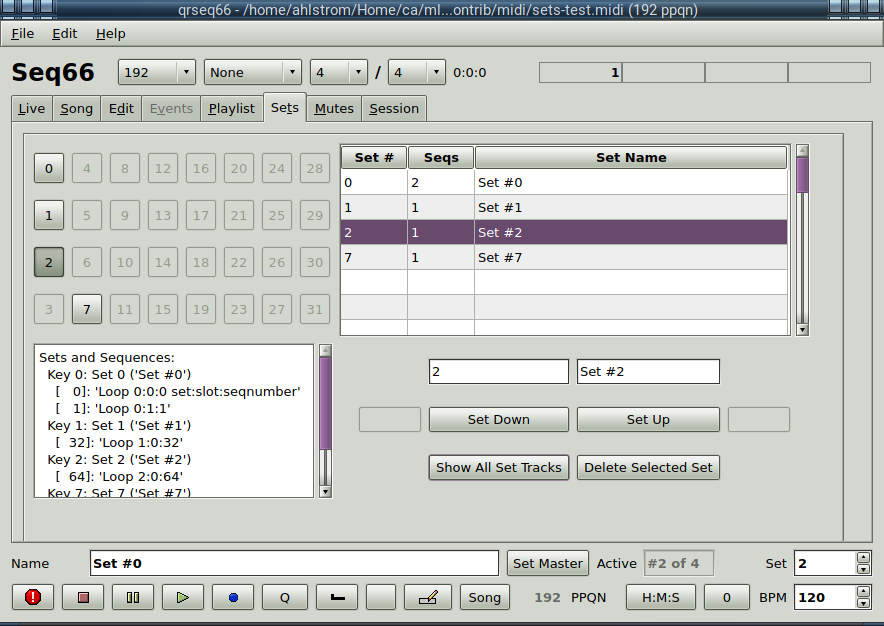
\includegraphics[scale=0.85]{tabs/sets/setmaster-tab.png}
   \caption{Sets Tab}
   \label{fig:setmaster_tab}
\end{figure}

   The operations that can be done consist of viewing the sets, making a
   screenset active, rearranging the sets, removing sets, and getting a survey of
   the contents of the sets.

   \setcounter{ItemCounter}{0}      % Reset the ItemCounter for this list.

   \itempar{Sets Grid}{set master!grid}
   The set grid is (presumably) always 4 x 8.  Like the mute-groups, there's not
   a lot of benefit supporting more sets.  The reader may wish to email us
   arguing for a different point of view.
   \index{play screen}
   This grid shows the sets that are
   present in the MIDI file, and allows one to choose which set is currently
   active (i.e. which is the "play screen").
   Click on it and it is active.
   Also remember that keystrokes (\texttt{[} and \texttt{]} by default)
 
   \itempar{Set List}{set master!list}
   The table at the right shows the set numbers, how many patterns/sequences are
   in each set, and the set name.  Eventually the set name will be editable.

   \itempar{Set Number/Name Fields}{set master!number/name}
   Eventually, these fields will be editable.

   \itempar{Set Up/Down Buttons}{set master!up/down buttons}
   These buttons allow the user to move the sets up and down.

   \itempar{Show All Set Tracks}{set master!show all set tracks}
   Clicking this button lists all the sets and their tracks in the edit box at
   the left. This functionality is provisional.

   \itempar{Delete Selected Set}{set master!delete selected set}
   Clicking this button deletes the set selected in the table above it.
   Note that the 0th set cannot be deleted.
   In \textsl{Seq66}, there must always be a set 0.

%-------------------------------------------------------------------------------
% vim: ts=3 sw=3 et ft=tex
%-------------------------------------------------------------------------------
